\section{Auswertung}

Alle gemessenen Werte der jeweiligen Versuchsdurchführung sind in den Tabellen \ref{tab:1} bis \ref{tab:3} angegeben. 

\subsection{Bestimmung der Schallgeschwindigkeit in Acryl}

Für die Bestimmung der Schallgeschwindigkeit in Acryl $c_{\text{acryl}}$ werden die Laufzeiten $\increment t$, sowie die Abstände $s$ aus Tabelle \ref{tab:1} und \ref{tab:2} verwendet.
Es gilt ganz allgemein nach Gleichung \eqref{eqn:WegvonSchallDurchEinMediumMitSchallgeschwindkeitCUndLaufzeitDeltaTWoebiDasBestimmtAuchAlsLichgeschwindgeitGesehenwerdenkannwennmankeineahnunghatundnichtdenkontextcheckt.}
\begin{equation*}
s = \frac{1}{2} c \cdot t \quad \to \quad 2s = c \cdot t,
\end{equation*}
damit liegt es nahe mit den Messwerten eine lineare Regression durchzuführen, um somit die Schallgeschwindigkeit zu erhalten.
Die allgemeine Form der Ausgleichsgeraden sieht folgendermaßen aus.
\begin{equation*}
y = ax + b
\end{equation*}
Durch einen \enquote{Polyfit} erster Ordnung mit Numpy \cite{numpy} ergeben sich die folgenden Parameter 
\begin{align*}
a &= \SI{2814.79(5441)}{\meter\per\second}, \\
b &= \SI{-5.64(169)}{\milli\meter}.
\end{align*}
Hierbei entspricht $a$ der Schallgeschwindigkeit $c$ in Acryl. Also ist 
\begin{equation}
    \label{eqn:1}
c_{\text{acryl}} = \SI{2814.79(5441)}{\meter\per\second}.
\end{equation}
Die Messwerte, sowie die Lineare Regression sind in der Abbildung \ref{fig:plot1} dargestellt.
\newline
Aus der ermittelten Schallgeschwindigkeit $c_{\text{acryl}}$ und den gemessenen Laufzeiten $\increment t$ lassen sich nun die theoretischen Abstände bis zur jeweiligen Fehlstelle bestimmen. 
Dabei gilt wieder die Gleichung \eqref{eqn:WegvonSchallDurchEinMediumMitSchallgeschwindkeitCUndLaufzeitDeltaTWoebiDasBestimmtAuchAlsLichgeschwindgeitGesehenwerdenkannwennmankeineahnunghatundnichtdenkontextcheckt.} und die dadurch bestimmten Abstände sind
in der Tabelle \ref{tab:wertewerte} notiert. Desweiteren sind die prozentuale Abweichung zwischen den gemessenen und theoretischen Abständen $s$ angegeben. 
\newpage
\begin{figure}
    \centering
    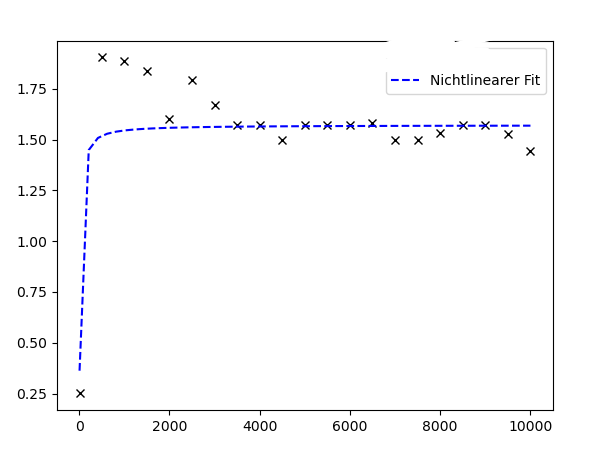
\includegraphics[width=\textwidth]{build/plot1.pdf}
    \caption{Messwerte mit linearer Regression zur Bestimmung der Schallgeschwindigkeit in Acryl.} 
    \label{fig:plot1}
\end{figure}

\begin{table}
    \centering
    \caption{Theoretische Bestimmung der Abstände zwischen der Oberfläche und den Fehlstellen mit der Beschriftung aus Abbildung \ref{fig:skizzeyo} sowie die prozentuale Abweichung zu den gemessenen Werten.}
    \label{tab:wertewerte}
    \begin{tabular}{c | c  c c c}
        \toprule
        Abstand & $s_{\text{gem}}$ [$\si{\milli\meter}$] &~& $s_{\text{theo}}$ [$\si{\milli\meter}$] & Abweichung $\increment s$ [$\si{\percent}$]\\
        \midrule
        \text{A}$'$ & $\SI{  6.70(10)}{}$ &~& $\SI{8.73(17)}{}$ &  $\SI{30.24(252)}{}$          \\ 
        \text{B}$'$ & $\SI{  9.65(10)}{}$ &~& $\SI{17.17(33)}{}$&  $\SI{77.93(344)}{}$           \\ 
        \text{C}$'$ & $\SI{ 22.60(10)}{}$ &~& $\SI{25.19(49)}{}$&  $\SI{11.47(215)}{}$           \\ 
        \text{D}$'$ & $\SI{ 30.55(10)}{}$ &~& $\SI{33.50(65)}{}$&  $\SI{9.64(212)}{}$           \\ 
        \text{E}$'$ & $\SI{ 38.70(10)}{}$ &~& $\SI{41.66(81)}{}$&  $\SI{7.65(208)}{}$           \\ 
        \text{F}$'$ & $\SI{ 45.95(10)}{}$ &~& $\SI{49.26(95)}{}$&  $\SI{7.20(207)}{}$           \\ 
        \text{G}$'$ & $\SI{ 53.65(10)}{}$ &~& $\SI{57.00(110)}{}$& $\SI{6.24(205)}{}$    \\ 
        \text{H}$'$ & $\SI{ 61.10(10)}{}$ &~& $\SI{64.74(125)}{}$& $\SI{5.96(205)}{}$    \\ 
        \text{I}$'$ & $\SI{ 54.15(10)}{}$ &~& $\SI{58.69(113)}{}$& $\SI{8.38(210)}{}$    \\ 
        \text{J}$'$ & $\SI{ 17.75(10)}{}$ &~& $\SI{19.84(38)}{}$ & $\SI{11.80(216)}{}$   \\ 
        \text{K}$'$ & $\SI{ 19.40(10)}{}$ &~& $\SI{21.39(41)}{}$ & $\SI{10.27(213)}{}$    \\
        \text{A}$'' $&  / &~& / & /\\
        \text{B}$'' $&  $\SI{67.70(10) }{}$&~&$\SI{66.01(128)}{}$&  $\SI{2.50(188)}{}$        \\ 
        \text{C}$'' $&  $\SI{54.75(10) }{}$&~&$\SI{57.98(112)}{}$&  $\SI{5.90(205)}{}$        \\ 
        \text{D}$'' $&  $\SI{46.80(10) }{}$&~&$\SI{49.82(96)}{}$ &  $\SI{6.46(206)}{}$       \\ 
        \text{E}$'' $&  $\SI{38.65(10) }{}$&~&$\SI{41.66(81)}{}$ &  $\SI{7.78(208)}{}$       \\ 
        \text{F}$'' $&  $\SI{30.30(10) }{}$&~&$\SI{32.79(63)}{}$ &  $\SI{8.23(209)}{}$       \\ 
        \text{G}$'' $&  $\SI{21.70(10) }{}$&~&$\SI{24.21(47)}{}$ &  $\SI{11.55(216)}{}$          \\ 
        \text{H}$'' $&  $\SI{13.25(10) }{}$&~&$\SI{15.20(30)}{}$ &  $\SI{14.72(222)}{}$          \\ 
        \text{I}$'' $&  $\SI{16.20(10) }{}$&~&$\SI{17.31(33)}{}$ &  $\SI{6.86(207)}{}$          \\ 
        \text{J}$'' $&  $\SI{61.20(10) }{}$&~&$\SI{64.74(125)}{}$&  $\SI{5.78(204)}{}$           \\ 
        \text{K}$'' $&  $\SI{59.55(10) }{}$&~&$\SI{62.63(121)}{}$&  $\SI{5.17(203)}{}$           \\ 
        
        
        
        
        
        
        
        
        
        
        
        \bottomrule
    \end{tabular}
\end{table}

\subsection{Messungen am Augenmodell}

Die gemessenen Spannungen, sowie Laufzeiten am Augenmodell sind in der Tabelle \ref{tab:3} angegeben. Zusätzlich sind die Schallgeschwindigkeiten der Linse $c_{\text{L}}$ und der Glaskörperflüssigkeit $c_{\text{GK}}$ gegeben mit
\begin{align*}
    c_{\text{L}} &= \SI{2500}{\meter\per\second},\\
    c_{\text{GK}} &= \SI{1410}{\meter\per\second}.
\end{align*}
Während der Versuchsdurchführung wurde ein momentanes Spannungsbild eingefangen. Dies ist in Abbildung \ref{fig:augewtf} gezeigt. Erkennbar sind also vier Peaks hinter der ausgehenden Spannung des Ultraschallsenders bei $t = \SI{0}{\second}$. Diese lassen sich
als die Grenzflächenübergänge zwischen 
\begin{equation*}
\text{Glaskörperflüssigkeit} \underbrace{\to \text{Iris}}_{\text{1.Peak}} \underbrace{\to \text{Linse}}_{\text{2.Peak}} \underbrace{\to \text{Glaskörperflüssigkeit}}_{\text{3.Peak}} \underbrace{\to \text{Retina}}_{\text{4.Peak}}
\end{equation*}
interpretieren. 

\begin{figure}
    \centering
    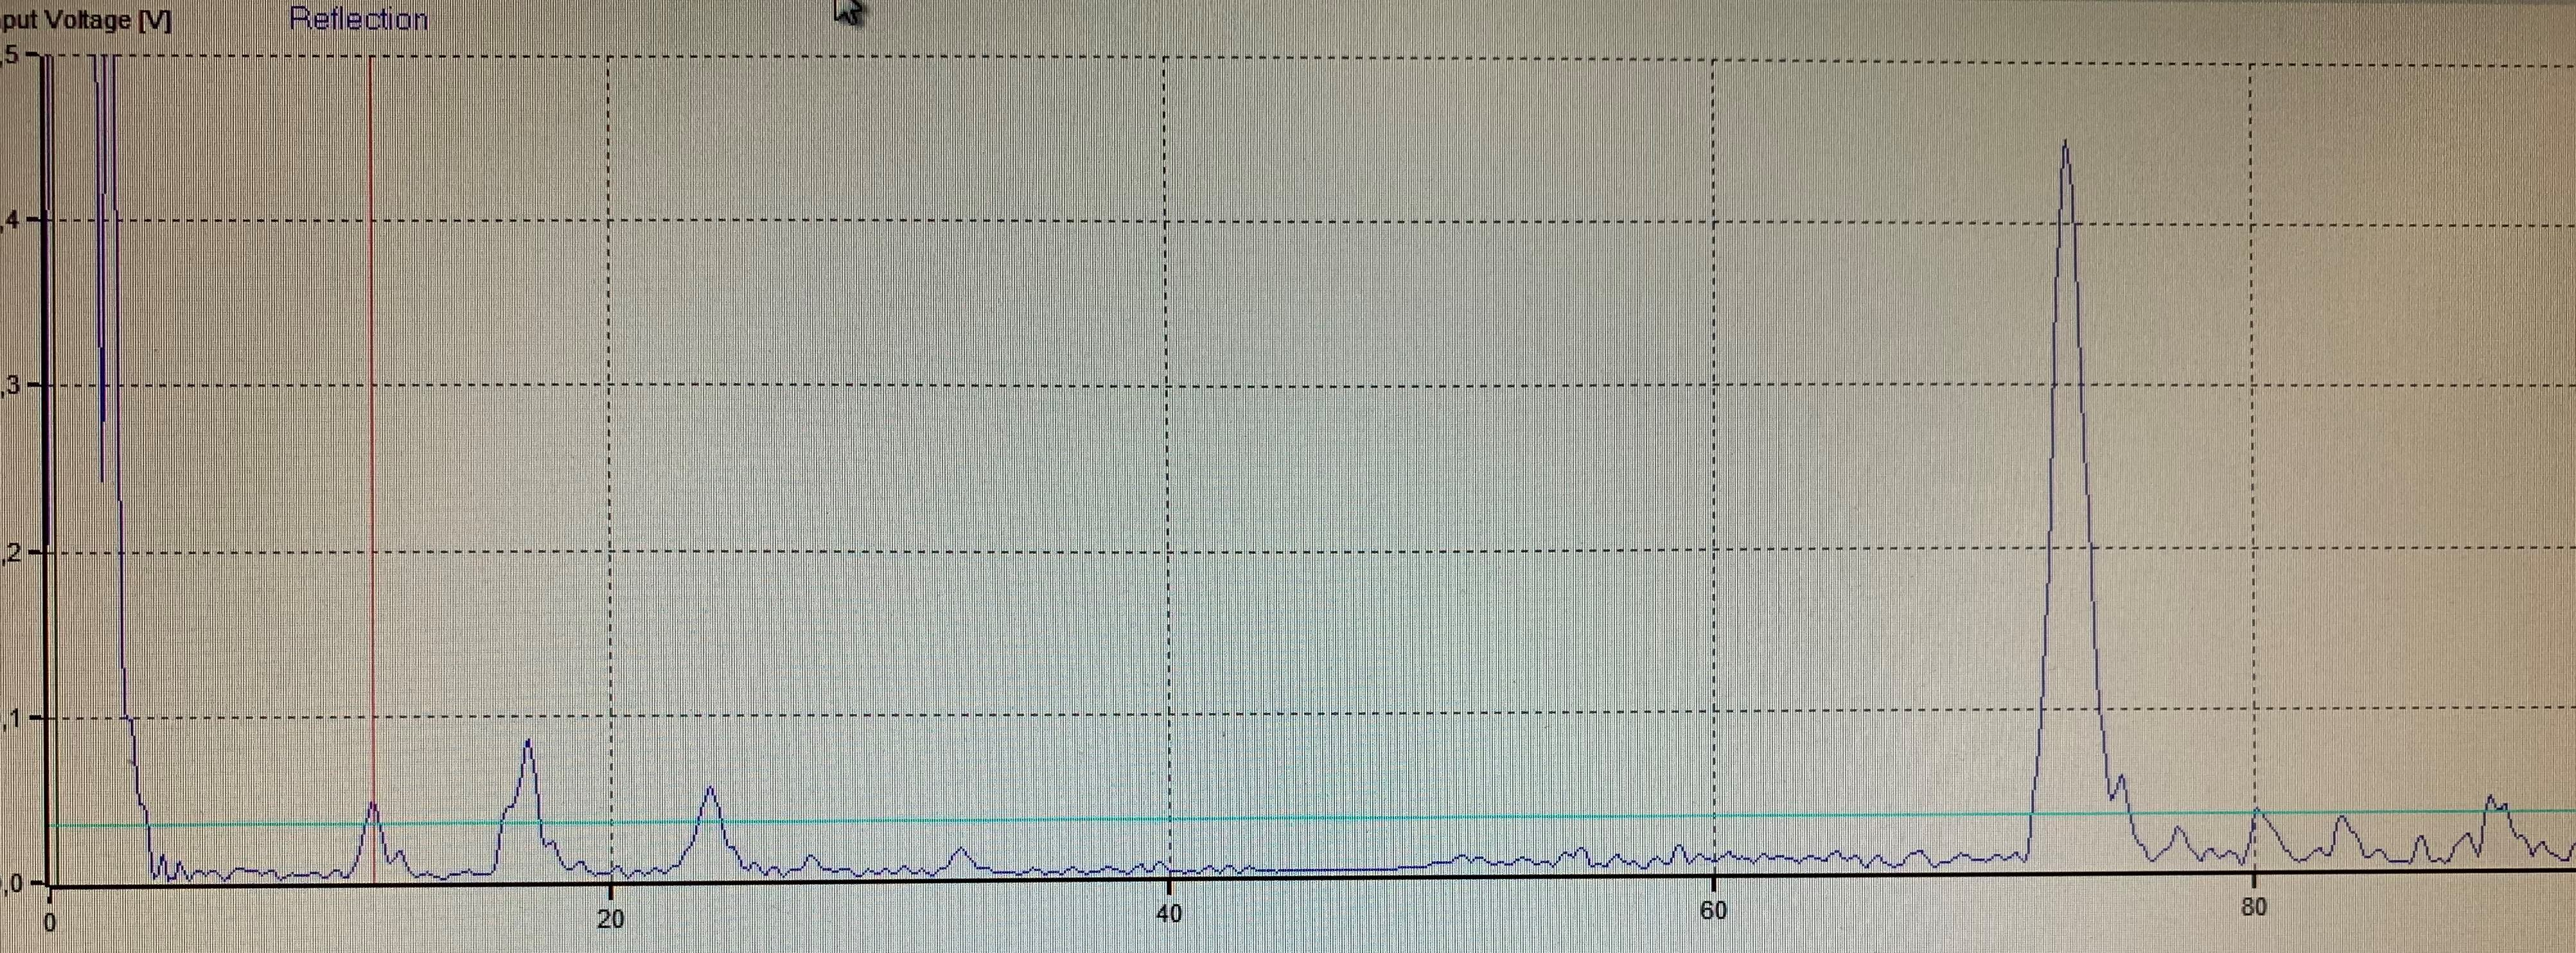
\includegraphics[width=\textwidth]{bilder/auge1.jpg}
    \caption{Laufzeit und Spannungsbild am Augenmodell mit den erkennbaren Peaks.} 
    \label{fig:augewtf}
\end{figure}
\FloatBarrier
\begin{flushleft}
Nun lassen sich die Abstände zwischen den einzelnen Bestandteilen des Augenmodells nach Abbildung \ref{fig:augeyo} ausrechnen. Dazu werden die oben genannten Schallgeschwindigkeiten des jeweiligen Mediums, sowie die Differenzen der Laufzeiten unter Verwendung der 
Gleichung \eqref{eqn:WegvonSchallDurchEinMediumMitSchallgeschwindkeitCUndLaufzeitDeltaTWoebiDasBestimmtAuchAlsLichgeschwindgeitGesehenwerdenkannwennmankeineahnunghatundnichtdenkontextcheckt.} genutzt.
\end{flushleft}
Die Ergebnisse sind in der Tabelle \ref{tab:4} aufgelistet.
\begin{table}
    \centering
    \caption{Errechnete Abstände im Augenmodell.}
    \label{tab:4}
    \begin{tabular}{c c}
        \toprule
        Abstand & $s$ [$\si{\milli\meter}$]  \\
        \midrule
        Sonde $\to$ Iris  &$\SI{8.11(7)}{}$\\
        Iris $\to$ Linse I  &$\SI{3.67(10)}{}$\\
        Linse I $\to$ Linse II &$\SI{8.50(18)}{}$\\
        Linse II $\to$ Retina &$\SI{34.83(10)}{}$\\
        \midrule
        Sonde $\to$ Linse I& $\SI{11.78(17)}{}$\\
        Sonde $\to$ Linse II& $\SI{20.36(35)}{}$\\
        Sonde $\to$ Retina& $\SI{55.19(45)}{}$\\    
    \end{tabular}
\end{table}


